% Options for packages loaded elsewhere
\PassOptionsToPackage{unicode}{hyperref}
\PassOptionsToPackage{hyphens}{url}
%
\documentclass[
]{book}
\usepackage{amsmath,amssymb}
\usepackage{lmodern}
\usepackage{iftex}
\ifPDFTeX
  \usepackage[T1]{fontenc}
  \usepackage[utf8]{inputenc}
  \usepackage{textcomp} % provide euro and other symbols
\else % if luatex or xetex
  \usepackage{unicode-math}
  \defaultfontfeatures{Scale=MatchLowercase}
  \defaultfontfeatures[\rmfamily]{Ligatures=TeX,Scale=1}
\fi
% Use upquote if available, for straight quotes in verbatim environments
\IfFileExists{upquote.sty}{\usepackage{upquote}}{}
\IfFileExists{microtype.sty}{% use microtype if available
  \usepackage[]{microtype}
  \UseMicrotypeSet[protrusion]{basicmath} % disable protrusion for tt fonts
}{}
\makeatletter
\@ifundefined{KOMAClassName}{% if non-KOMA class
  \IfFileExists{parskip.sty}{%
    \usepackage{parskip}
  }{% else
    \setlength{\parindent}{0pt}
    \setlength{\parskip}{6pt plus 2pt minus 1pt}}
}{% if KOMA class
  \KOMAoptions{parskip=half}}
\makeatother
\usepackage{xcolor}
\IfFileExists{xurl.sty}{\usepackage{xurl}}{} % add URL line breaks if available
\IfFileExists{bookmark.sty}{\usepackage{bookmark}}{\usepackage{hyperref}}
\hypersetup{
  pdftitle={mashup: N-mixture models},
  pdfauthor={Cord Phelps},
  hidelinks,
  pdfcreator={LaTeX via pandoc}}
\urlstyle{same} % disable monospaced font for URLs
\usepackage{color}
\usepackage{fancyvrb}
\newcommand{\VerbBar}{|}
\newcommand{\VERB}{\Verb[commandchars=\\\{\}]}
\DefineVerbatimEnvironment{Highlighting}{Verbatim}{commandchars=\\\{\}}
% Add ',fontsize=\small' for more characters per line
\usepackage{framed}
\definecolor{shadecolor}{RGB}{248,248,248}
\newenvironment{Shaded}{\begin{snugshade}}{\end{snugshade}}
\newcommand{\AlertTok}[1]{\textcolor[rgb]{0.94,0.16,0.16}{#1}}
\newcommand{\AnnotationTok}[1]{\textcolor[rgb]{0.56,0.35,0.01}{\textbf{\textit{#1}}}}
\newcommand{\AttributeTok}[1]{\textcolor[rgb]{0.77,0.63,0.00}{#1}}
\newcommand{\BaseNTok}[1]{\textcolor[rgb]{0.00,0.00,0.81}{#1}}
\newcommand{\BuiltInTok}[1]{#1}
\newcommand{\CharTok}[1]{\textcolor[rgb]{0.31,0.60,0.02}{#1}}
\newcommand{\CommentTok}[1]{\textcolor[rgb]{0.56,0.35,0.01}{\textit{#1}}}
\newcommand{\CommentVarTok}[1]{\textcolor[rgb]{0.56,0.35,0.01}{\textbf{\textit{#1}}}}
\newcommand{\ConstantTok}[1]{\textcolor[rgb]{0.00,0.00,0.00}{#1}}
\newcommand{\ControlFlowTok}[1]{\textcolor[rgb]{0.13,0.29,0.53}{\textbf{#1}}}
\newcommand{\DataTypeTok}[1]{\textcolor[rgb]{0.13,0.29,0.53}{#1}}
\newcommand{\DecValTok}[1]{\textcolor[rgb]{0.00,0.00,0.81}{#1}}
\newcommand{\DocumentationTok}[1]{\textcolor[rgb]{0.56,0.35,0.01}{\textbf{\textit{#1}}}}
\newcommand{\ErrorTok}[1]{\textcolor[rgb]{0.64,0.00,0.00}{\textbf{#1}}}
\newcommand{\ExtensionTok}[1]{#1}
\newcommand{\FloatTok}[1]{\textcolor[rgb]{0.00,0.00,0.81}{#1}}
\newcommand{\FunctionTok}[1]{\textcolor[rgb]{0.00,0.00,0.00}{#1}}
\newcommand{\ImportTok}[1]{#1}
\newcommand{\InformationTok}[1]{\textcolor[rgb]{0.56,0.35,0.01}{\textbf{\textit{#1}}}}
\newcommand{\KeywordTok}[1]{\textcolor[rgb]{0.13,0.29,0.53}{\textbf{#1}}}
\newcommand{\NormalTok}[1]{#1}
\newcommand{\OperatorTok}[1]{\textcolor[rgb]{0.81,0.36,0.00}{\textbf{#1}}}
\newcommand{\OtherTok}[1]{\textcolor[rgb]{0.56,0.35,0.01}{#1}}
\newcommand{\PreprocessorTok}[1]{\textcolor[rgb]{0.56,0.35,0.01}{\textit{#1}}}
\newcommand{\RegionMarkerTok}[1]{#1}
\newcommand{\SpecialCharTok}[1]{\textcolor[rgb]{0.00,0.00,0.00}{#1}}
\newcommand{\SpecialStringTok}[1]{\textcolor[rgb]{0.31,0.60,0.02}{#1}}
\newcommand{\StringTok}[1]{\textcolor[rgb]{0.31,0.60,0.02}{#1}}
\newcommand{\VariableTok}[1]{\textcolor[rgb]{0.00,0.00,0.00}{#1}}
\newcommand{\VerbatimStringTok}[1]{\textcolor[rgb]{0.31,0.60,0.02}{#1}}
\newcommand{\WarningTok}[1]{\textcolor[rgb]{0.56,0.35,0.01}{\textbf{\textit{#1}}}}
\usepackage{longtable,booktabs,array}
\usepackage{calc} % for calculating minipage widths
% Correct order of tables after \paragraph or \subparagraph
\usepackage{etoolbox}
\makeatletter
\patchcmd\longtable{\par}{\if@noskipsec\mbox{}\fi\par}{}{}
\makeatother
% Allow footnotes in longtable head/foot
\IfFileExists{footnotehyper.sty}{\usepackage{footnotehyper}}{\usepackage{footnote}}
\makesavenoteenv{longtable}
\usepackage{graphicx}
\makeatletter
\def\maxwidth{\ifdim\Gin@nat@width>\linewidth\linewidth\else\Gin@nat@width\fi}
\def\maxheight{\ifdim\Gin@nat@height>\textheight\textheight\else\Gin@nat@height\fi}
\makeatother
% Scale images if necessary, so that they will not overflow the page
% margins by default, and it is still possible to overwrite the defaults
% using explicit options in \includegraphics[width, height, ...]{}
\setkeys{Gin}{width=\maxwidth,height=\maxheight,keepaspectratio}
% Set default figure placement to htbp
\makeatletter
\def\fps@figure{htbp}
\makeatother
\setlength{\emergencystretch}{3em} % prevent overfull lines
\providecommand{\tightlist}{%
  \setlength{\itemsep}{0pt}\setlength{\parskip}{0pt}}
\setcounter{secnumdepth}{5}
\usepackage{booktabs}
\usepackage{amsthm}
\makeatletter
\def\thm@space@setup{%
  \thm@preskip=8pt plus 2pt minus 4pt
  \thm@postskip=\thm@preskip
}
\makeatother
\ifLuaTeX
  \usepackage{selnolig}  % disable illegal ligatures
\fi
\usepackage[]{natbib}
\bibliographystyle{apalike}

\title{mashup: N-mixture models}
\author{Cord Phelps}
\date{August 2021}

\begin{document}
\maketitle

{
\setcounter{tocdepth}{1}
\tableofcontents
}
\hypertarget{preface}{%
\chapter{preface}\label{preface}}

Not finding literature on the estimation of spider populations in vineyard canopy, I fall back on available descriptions of non-invasive sampling strategy and analytical techniques for animal populations in general. Specifically, the journal article Comparison of Two Sampling Methods to Estimate the Abundance of Lucanus cervus with Application of n-Mixture Models \citep{f11101085} leads to a review and investigation of N-mixture models by Javier Fernández-López \citep{fernandez-lopez_n-mixture_2020}.

This project is a mashup that follows Javier's work, first by translating his Spanish to English using google translate \citep{noauthor_google_nodate}, and then by using his recommended techniques to apply n-mixture modelling to my vineyard spider data.

\hypertarget{n-mixture-model-tutorial}{%
\chapter{n-mixture model tutorial}\label{n-mixture-model-tutorial}}

\begin{col}{0.45\textwidth}
Este tutorial está basado principalmente en el capítulo 6 del libro Applied Hierarchical Modeling in Ecology Analysis of distribution, abundance and species richness in R and BUGS de Marc Kéry y J. Andrew Royle (Kéry and Royle 2016). Existen otros buenos tutoriales como este de M.E. Colvin o estos del Cornell Lab of Ornitology que también han sido consultados.

\end{col}

\begin{col}{0.05\textwidth}
~

\end{col}

\begin{col}{0.45\textwidth}
This tutorial is primarily based on Chapter 6 of the book Applied Hierarchical Modeling in Ecology Analysis of distribution, abundance and species richness in R and BUGS by Marc Kéry and J. Andrew Royle (Kéry and Royle 2016). There are other good tutorials like this one from M.E. Colvin or these from the Cornell Lab of Ornitology that have also been consulted.

\end{col}

\hypertarget{intro}{%
\chapter{Introduction}\label{intro}}

\begin{col}{0.45\textwidth}
La abundancia o el número de individuos de una población es un parámetro clave para conocer el estado de la misma y poder realizar una correcta gestión (Krebs 2009). Sin embargo, estimar el número total de individuos que componenen una población, N, no es tarea sencilla. Para aproximarse a ese número se pueden diseñar muestreos que nos permitan obtener un índice de abundancia I, que puede definirse como ``cantidades que reflejan variaciones temporales o espaciales del tamaño de las poblaciones sin conocer realmente su verdadero tamaño'' (Tellería 2012). De forma general, se considera que

\end{col}

\begin{col}{0.05\textwidth}
~

\end{col}

\begin{col}{0.45\textwidth}
The abundance or the number of individuals in a population is a key parameter to know its status and to be able to carry out proper management (Krebs 2009). However, estimating the total number of individuals that make up a population, N, is not an easy task. To approach this number, samples can be designed that allow us to obtain an abundance index I, which can be defined as ``quantities that reflect temporal or spatial variations in the size of the populations without really knowing their true size'' (Tellería 2012). In general, it is considered that

\end{col}

\[ I = p * N \]

\begin{col}{0.45\textwidth}
donde N es el número total de individuos de una población, I el índice de abundancia (un conteo de individuos que hayamos obtenido durante el muestreo, por ejemplo) y p sería la detectabilidad o capturabilidad, la eficacia que tenemos para detectar individuos durante los muestreos. Si logramos mantener constante esa p, el índice puede ser útil para realizar comparaciones de abundancia en el espacio-tiempo. Sin embargo, muchas veces la detectabilidad está condicionada por covariables que impiden mantenerla constante (muestreos realizados en diferentes épocas del año, lugares con más o menos visibilidad, etc.). Conocer esta p y sus variaciones nos permitiría estimar el número absoluto de individuos N, lo cual puede ser esencial en especies en críticamente amenazadas. Algunas aproximaciones como la captura-marcaje-recaptura se basan en la identificación individual de los individuos para estimar esta detectabilidad p y poder así obtener abundancias absolutas (Efford 2004), pero esta metodología suele ser costosa de implementar, ya que requiere una caprura y un manejo de los individuos de estudio que no es siempre posible.

\end{col}

\begin{col}{0.05\textwidth}
~

\end{col}

\begin{col}{0.45\textwidth}
where N is the total number of individuals in a population, I the abundance index (a count of individuals that we have obtained during the sampling, for example) and p would be the detectability or catchability, the efficiency we have in detecting individuals during the samplings. If we can keep that p constant, the index can be useful for making comparisons of abundance in space-time. However, detectability is often conditioned by covariates that prevent it from being constant (samplings carried out at different times of the year, places with more or less visibility, etc.). Knowing this p and its variations would allow us to estimate the absolute number of individuals N, which may be essential in critically endangered species. Some approaches such as capture-mark-recapture are based on the individual identification of individuals to estimate this detectability and thus be able to obtain absolute abundances (Efford 2004), but this methodology is usually expensive to implement, since it requires capriation and management. of study individuals that is not always possible.

\end{col}

\begin{col}{0.45\textwidth}
Los N-mixture models, modelos de mezclas o modelo de conteos (Royle 2004) nos permiten estimar la abundancia de una especie a partir de muestreos repetidos. Estos modelos tienen una estructura jerárquica (Kéry and Royle 2016) y estiman a la vez la abundancia y la detectabilidad/capturabilidad de la especie de estudio a partir de conteos repetidos t ocasiones en n sitios diferentes.

En el siguiente tutorial se pretende comprender las generalidades de los N-mixture models a partir de la simulación de dos sencillos escenarios utilizando el lenguaje R y el paquete unmarked (Fiske and Chandler 2011).

\end{col}

\begin{col}{0.05\textwidth}
~

\end{col}

\begin{col}{0.45\textwidth}
The N-mixture models, mixture models or counting models (Royle 2004) allow us to estimate the abundance of a species from repeated samplings. These models have a hierarchical structure (Kéry and Royle 2016) and estimate both the abundance and the detectability / catchability of the study species from repeated counts t times at n different sites.

The following tutorial aims to understand the generalities of the N-mixture models from the simulation of two simple scenarios using the R language and the unmarked package (Fiske and Chandler 2011).

\end{col}

\hypertarget{gen}{%
\chapter{N mixture models: In General}\label{gen}}

\begin{col}{0.45\textwidth}
Pongamos que salimos al campo a buscar ciervos \emph{(Cervus elaphus)}.

De forma general, se podría afirmar que si detectamos un individuo de ciervo durante el muestreo, la especie está presente en ese lugar y en ese momento (asumimos que conocemos bien la especie y que no hay posibilidad de obtener falsos positivos, esto es, confundir otras especies con individuos de ciervo, por ejemplo). Sin embargo, el hecho de no detectarla puede estar indicándonos dos cosas:

\begin{enumerate}
\def\labelenumi{\arabic{enumi}.}
\item
  Que la especie \textbf{no esté presente} en ese lugar porque el hábitat no es el adecuado, o la especie se haya extinguido, etc. Esto sería un verdadero negativo.
\item
  Que la especie \textbf{si esté presente pero no hayamos sido capaces de detectarla} (hemos ido a muestrear al medio día y solo tiene actividad crepuscular, por ejemplo). Esto sería un falso negativo.
\end{enumerate}

Los N-mixture models son capaces de tener en cuenta la posibilidad de cometer falsos negativos cuando muestreamos varias ocasiones los mismos sitios. Tienen en cuenta dos procesos:

\begin{itemize}
\tightlist
\item
  Un proceso (o submodelo) que determina la abundancia de la especie. En inglés suele denominarse state process.
\item
  Un proceso (o submodelo) que determina la probabilidad de detección/observación de la especie. En inglés observational process.
\end{itemize}

Estos modelos suelen denominarse modelos jerárquicos ya que el proceso de detección depende en parte del proceso de abundancia. A continuación simularemos una serie de escenarios a modo de ejemplo para entender un poco mejor los N-mixture models.

\end{col}

\begin{col}{0.05\textwidth}
~

\end{col}

\begin{col}{0.45\textwidth}
Let's say we go out into the field to look for deer \emph{(Cervus elaphus)}.

In general, it could be stated that if we detect an individual deer during the sampling, the species is present in that place and at that time (we assume that we know the species well and that there is no possibility of obtaining false positives, that is, confusing other species with deer individuals, for example). However, the fact of not detecting it may be indicating two things:

\begin{enumerate}
\def\labelenumi{\arabic{enumi}.}
\item
  That the species \textbf{is not present} in that place because the habitat is not adequate, or the species has become extinct, etc. This would be a real negative.
\item
  That the species \textbf{is present but we have not been able to detect it} (we have gone to sample at noon and it only has twilight activity, for example). This would be a false negative.
\end{enumerate}

The N-mixture models are able to take into account the possibility of committing false negatives when we repeatedly sample the same sites. They take into account two processes:

\begin{itemize}
\tightlist
\item
  A process (or sub-model) that determines the abundance of the species. In English it is usually called the state process.
\item
  A process (or sub-model) that determines the probability of detection / observation of the species. In English observational process.
\end{itemize}

These models are often called hierarchical models since the detection process depends in part on the abundance process. Below we will simulate a series of example scenarios to understand the N-mixture models a little better.

\end{col}

\hypertarget{simWithout}{%
\chapter{Simulation of a population and a sampling WITHOUT covariates}\label{simWithout}}

\begin{col}{0.45\textwidth}
Con ayuda de R, vamos a simular una población de ciervos que se distribuye en un área de 100 km2 (100 cuadrados de 1 km de lado)

\end{col}

\begin{col}{0.05\textwidth}
~

\end{col}

\begin{col}{0.45\textwidth}
With the help of R, we are going to simulate a deer population that is distributed in an area of 100 km2 (100 squares of 1 km on each side)

\end{col}

\begin{Shaded}
\begin{Highlighting}[]
\FunctionTok{set.seed}\NormalTok{(}\DecValTok{1}\NormalTok{) }\CommentTok{\# ajustamos una "semilla"" para controlar la repetibilidad }
\CommentTok{\# Con el paquete "raster" creamos una cuadrícula de 10x10}
\FunctionTok{library}\NormalTok{(raster)}
\NormalTok{sarea }\OtherTok{\textless{}{-}} \FunctionTok{raster}\NormalTok{(}\AttributeTok{nrows =} \DecValTok{10}\NormalTok{, }\AttributeTok{ncols =} \DecValTok{10}\NormalTok{, }\AttributeTok{xmn =} \DecValTok{0}\NormalTok{, }\AttributeTok{xmx =} \DecValTok{10}\NormalTok{, }\AttributeTok{ymn =} \DecValTok{0}\NormalTok{, }\AttributeTok{ymx =} \DecValTok{10}\NormalTok{)}
\end{Highlighting}
\end{Shaded}

\begin{col}{0.45\textwidth}
Este área de momento está vacía, por lo que tendremos que ``llenarla'' de ciervos virtuales (proceso de abundancia, o state process). Podemos utilizar una distribución de Poisson para ``esparcir'' nuestros ciervos simulados en el área de estudio. Esta distrubución es una de las más comunmente utilizadas en el estudio de abundancias. La distribución de Poisson maneja la frecuencia con la que un evento ocurre en un intervalo específico. Consta de un único parámetro llamado lambda λ que determina el número de eventos que ocurren normalmente en ese intervalo.

\end{col}

\begin{col}{0.05\textwidth}
~

\end{col}

\begin{col}{0.45\textwidth}
This area is currently empty, so we will have to ``fill'' it with virtual deer (abundance process, or state process). We can use a Poisson distribution to ``spread'' our simulated deer in the study area. This distribution is one of the most commonly used in the study of abundances. The Poisson distribution handles the frequency with which an event occurs in a specific interval. It consists of a single parameter called lambda λ that determines the number of events that normally occur in that interval.

\end{col}

\begin{Shaded}
\begin{Highlighting}[]
\CommentTok{\# generate a random poisson distribution, 10000 values}
\NormalTok{poissonVector }\OtherTok{\textless{}{-}} \FunctionTok{rpois}\NormalTok{(}\AttributeTok{n =} \DecValTok{10000}\NormalTok{, }\AttributeTok{lambda =} \DecValTok{4}\NormalTok{)}
\CommentTok{\# convert the vector into a df}
\NormalTok{df }\OtherTok{\textless{}{-}} \FunctionTok{data.frame}\NormalTok{(}\AttributeTok{poissonCount =}\NormalTok{ poissonVector)}

\NormalTok{noPlot }\OtherTok{\textless{}{-}} \FunctionTok{ggplot}\NormalTok{(}\AttributeTok{data=}\NormalTok{df, }\FunctionTok{aes}\NormalTok{(}\AttributeTok{x =}\NormalTok{ poissonCount)) }\SpecialCharTok{+}
  \FunctionTok{geom\_histogram}\NormalTok{(}\AttributeTok{bins =} \DecValTok{14}\NormalTok{, }\AttributeTok{color =} \StringTok{"black"}\NormalTok{, }\AttributeTok{fill=}\StringTok{"white"}\NormalTok{) }\SpecialCharTok{+}
  \FunctionTok{theme\_bw}\NormalTok{() }\SpecialCharTok{+}
  \FunctionTok{labs}\NormalTok{( }\AttributeTok{x =} \StringTok{"poisson value (count)"}\NormalTok{, }
        \AttributeTok{y =} \StringTok{"occurrences (frequency)"}\NormalTok{, }
        \AttributeTok{title =} \StringTok{"poisson distribution}\SpecialCharTok{\textbackslash{}n}\StringTok{lambda = 4"}\NormalTok{)}
\end{Highlighting}
\end{Shaded}

\begin{col}{0.45\textwidth}
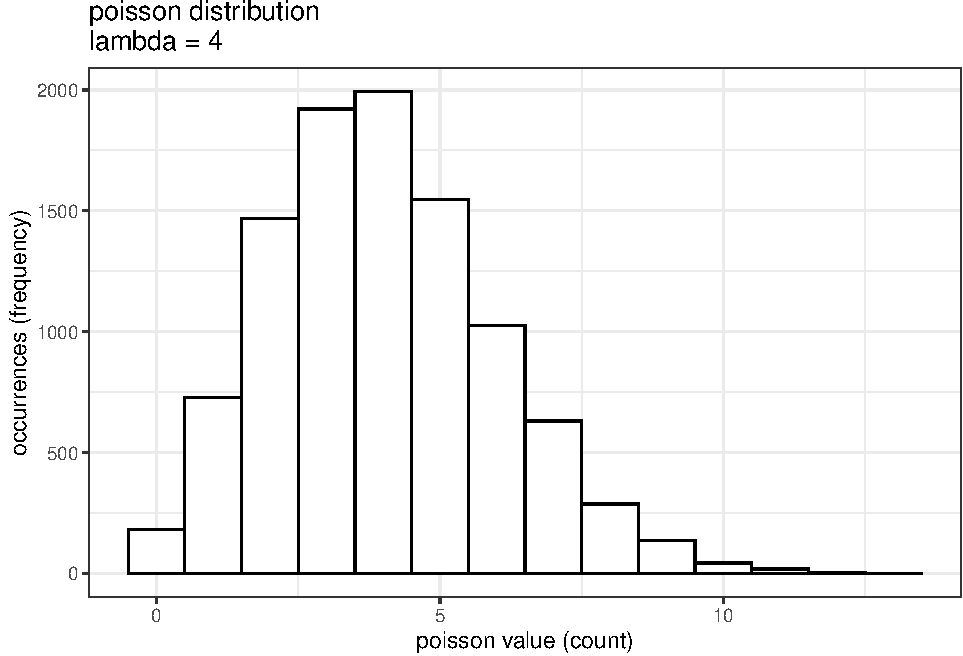
\includegraphics{bookdown-demo_files/figure-latex/gg1-1.pdf}

\end{col}

\begin{col}{0.05\textwidth}
~

\end{col}

\begin{col}{0.45\textwidth}
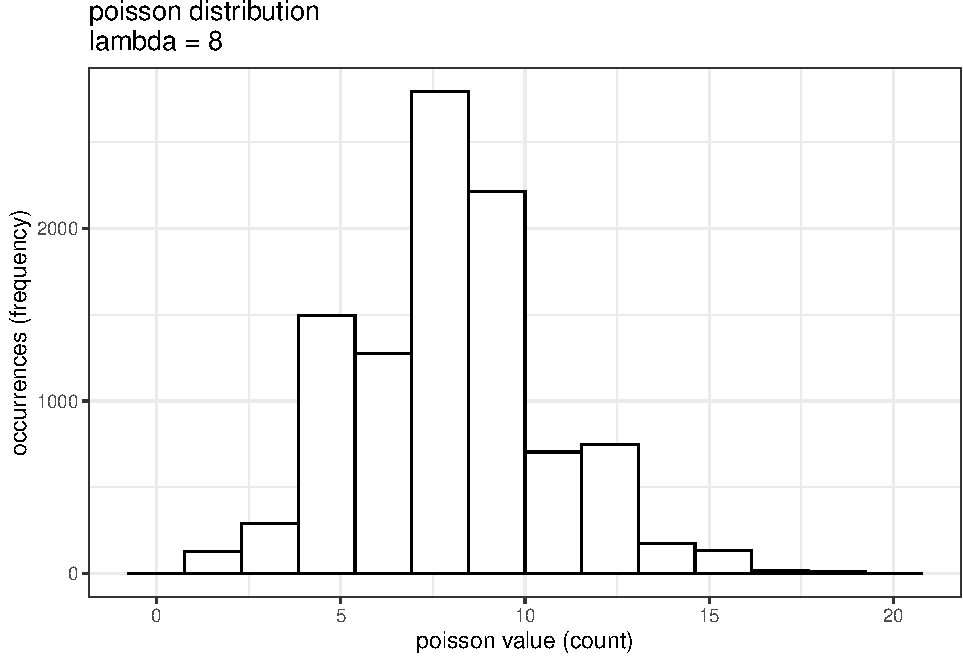
\includegraphics{bookdown-demo_files/figure-latex/gg2-1.pdf}

\end{col}

\begin{col}{0.45\textwidth}
En nuestro caso, el intervalo una unidad espacial, una cuadrícula, mientras que el evento será la presencia de un ciervo. El parámetro λ será la ``abundancia esperada'', esto es, la abundancia media por cuadrícula. El número y la distribución de los ciervos virtuales que colocaremos en nuestro área de estudio vendrá determinado por una distribución de Poisson con λ=4:

\end{col}

\begin{col}{0.05\textwidth}
~

\end{col}

\begin{col}{0.45\textwidth}
In our case, the interval will be a spatial unit, a grid, while the event will be the presence of a deer. The parameter λ will be the ``expected abundance'', that is, the mean abundance per grid. The number and distribution of virtual deer that we will place in our study area will be determined by a Poisson distribution with λ = 4:

\end{col}

\[ N_{i} \sim Poisson(λ) \]

\begin{col}{0.45\textwidth}
siendo \(N_{i}\) el número total de individuos en la celda i.

Como podemos ver en el histograma de la izquierda, los valores más probables serán 3 o 4 ciervos, aunque variarán entre cero y 14 aproximadamente (aunque este útimo valor será muy poco probable).

\end{col}

\begin{col}{0.05\textwidth}
~

\end{col}

\begin{col}{0.45\textwidth}
where \(N_{i}\) is the total number of individuals in cell i.

As we can see in the histogram on the left, the most probable values will be 3 or 4 deer, although they will vary between zero and 14 approximately (although this last value will be very unlikely).

\end{col}

\begin{Shaded}
\begin{Highlighting}[]
\CommentTok{\# Seleccionamos el lambda deseado}
\NormalTok{lambda }\OtherTok{\textless{}{-}} \DecValTok{4}

\CommentTok{\# Generamos 100 números aleatorios obtenidos de una distribucion}
\CommentTok{\# de Poisson con una lambda = 4}
\NormalTok{sarea[] }\OtherTok{\textless{}{-}} \FunctionTok{rpois}\NormalTok{(}\DecValTok{100}\NormalTok{, lambda)  }

\CommentTok{\# plot(sarea)}
\end{Highlighting}
\end{Shaded}

\begin{Shaded}
\begin{Highlighting}[]
\CommentTok{\# extract S4 data and build vector}
\NormalTok{area.vector }\OtherTok{\textless{}{-}} \FunctionTok{as.vector}\NormalTok{(sarea)}
\CommentTok{\# convert to matrix}
\NormalTok{area.matrix }\OtherTok{\textless{}{-}} \FunctionTok{matrix}\NormalTok{(area.vector, }\AttributeTok{byrow=}\NormalTok{T, }\AttributeTok{nrow=}\DecValTok{10}\NormalTok{, }\AttributeTok{ncol=}\DecValTok{10}\NormalTok{)}
\CommentTok{\# reverse the rows (so we can compare plots)}
\NormalTok{area.matrix }\OtherTok{\textless{}{-}} \FunctionTok{apply}\NormalTok{(area.matrix,}\DecValTok{2}\NormalTok{,rev)}
\FunctionTok{colnames}\NormalTok{(area.matrix) }\OtherTok{\textless{}{-}} \FunctionTok{c}\NormalTok{(}\DecValTok{1}\NormalTok{,}\DecValTok{2}\NormalTok{,}\DecValTok{3}\NormalTok{,}\DecValTok{4}\NormalTok{,}\DecValTok{5}\NormalTok{,}\DecValTok{6}\NormalTok{,}\DecValTok{7}\NormalTok{,}\DecValTok{8}\NormalTok{,}\DecValTok{9}\NormalTok{,}\DecValTok{10}\NormalTok{)}
\FunctionTok{rownames}\NormalTok{(area.matrix) }\OtherTok{\textless{}{-}} \FunctionTok{c}\NormalTok{(}\DecValTok{1}\NormalTok{,}\DecValTok{2}\NormalTok{,}\DecValTok{3}\NormalTok{,}\DecValTok{4}\NormalTok{,}\DecValTok{5}\NormalTok{,}\DecValTok{6}\NormalTok{,}\DecValTok{7}\NormalTok{,}\DecValTok{8}\NormalTok{,}\DecValTok{9}\NormalTok{,}\DecValTok{10}\NormalTok{)}

\NormalTok{longData}\OtherTok{\textless{}{-}}\FunctionTok{melt}\NormalTok{(area.matrix)}
\NormalTok{longData}\OtherTok{\textless{}{-}}\NormalTok{longData[longData}\SpecialCharTok{$}\NormalTok{value}\SpecialCharTok{!=}\DecValTok{0}\NormalTok{,]}

\NormalTok{noPlot }\OtherTok{\textless{}{-}} \FunctionTok{ggplot}\NormalTok{(longData, }\FunctionTok{aes}\NormalTok{(}\AttributeTok{x =}\NormalTok{ Var2, }\AttributeTok{y =}\NormalTok{ Var1)) }\SpecialCharTok{+} 
  \FunctionTok{geom\_raster}\NormalTok{(}\FunctionTok{aes}\NormalTok{(}\AttributeTok{fill=}\NormalTok{value)) }\SpecialCharTok{+} 
  \FunctionTok{scale\_fill\_gradientn}\NormalTok{(}\AttributeTok{colors=}\FunctionTok{rev}\NormalTok{(}\FunctionTok{terrain.colors}\NormalTok{(}\DecValTok{12}\NormalTok{))) }\SpecialCharTok{+}
  \FunctionTok{theme\_bw}\NormalTok{() }
\end{Highlighting}
\end{Shaded}

\begin{col}{0.45\textwidth}
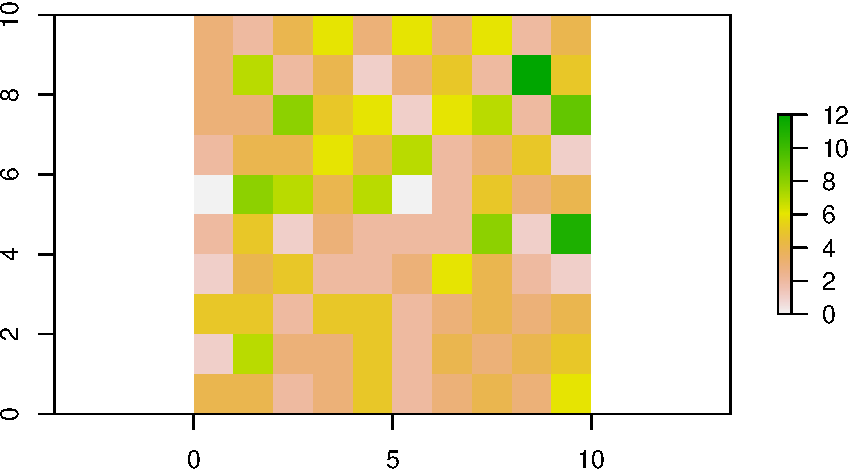
\includegraphics{bookdown-demo_files/figure-latex/area1-1.pdf}

\end{col}

\begin{col}{0.05\textwidth}
~

\end{col}

\begin{col}{0.45\textwidth}
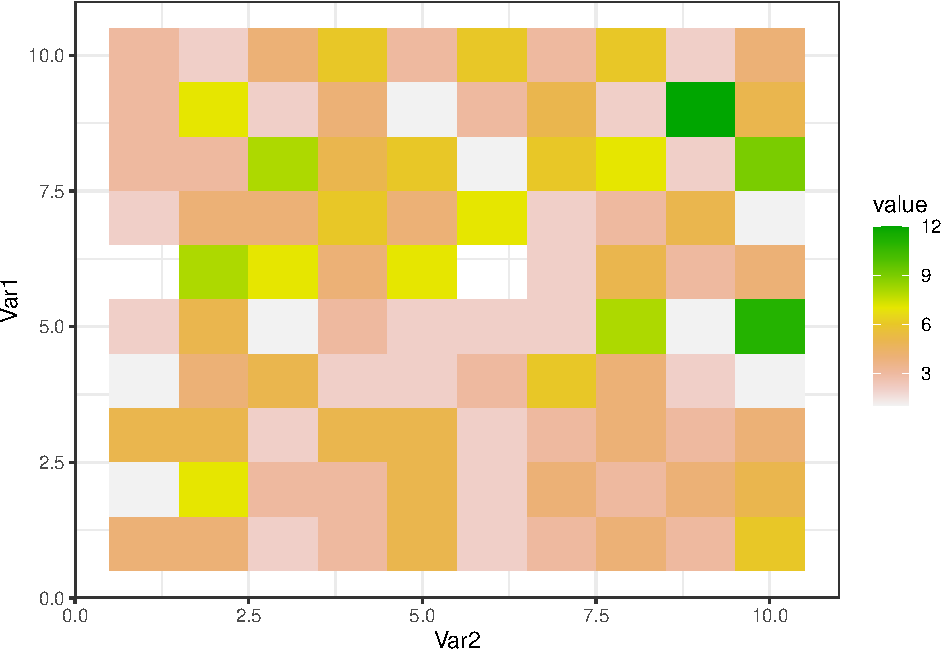
\includegraphics{bookdown-demo_files/figure-latex/area2-1.pdf}

\end{col}

\begin{col}{0.45\textwidth}
donde

\end{col}

\begin{col}{0.05\textwidth}
~

\end{col}

\begin{col}{0.45\textwidth}
where

\end{col}

\hypertarget{ref}{%
\chapter{references}\label{ref}}

Below is a Div containing three child Divs side by side. The Div
in the middle is empty, just to add more space between the left
and right Divs.

\begin{col}{0.45\textwidth}
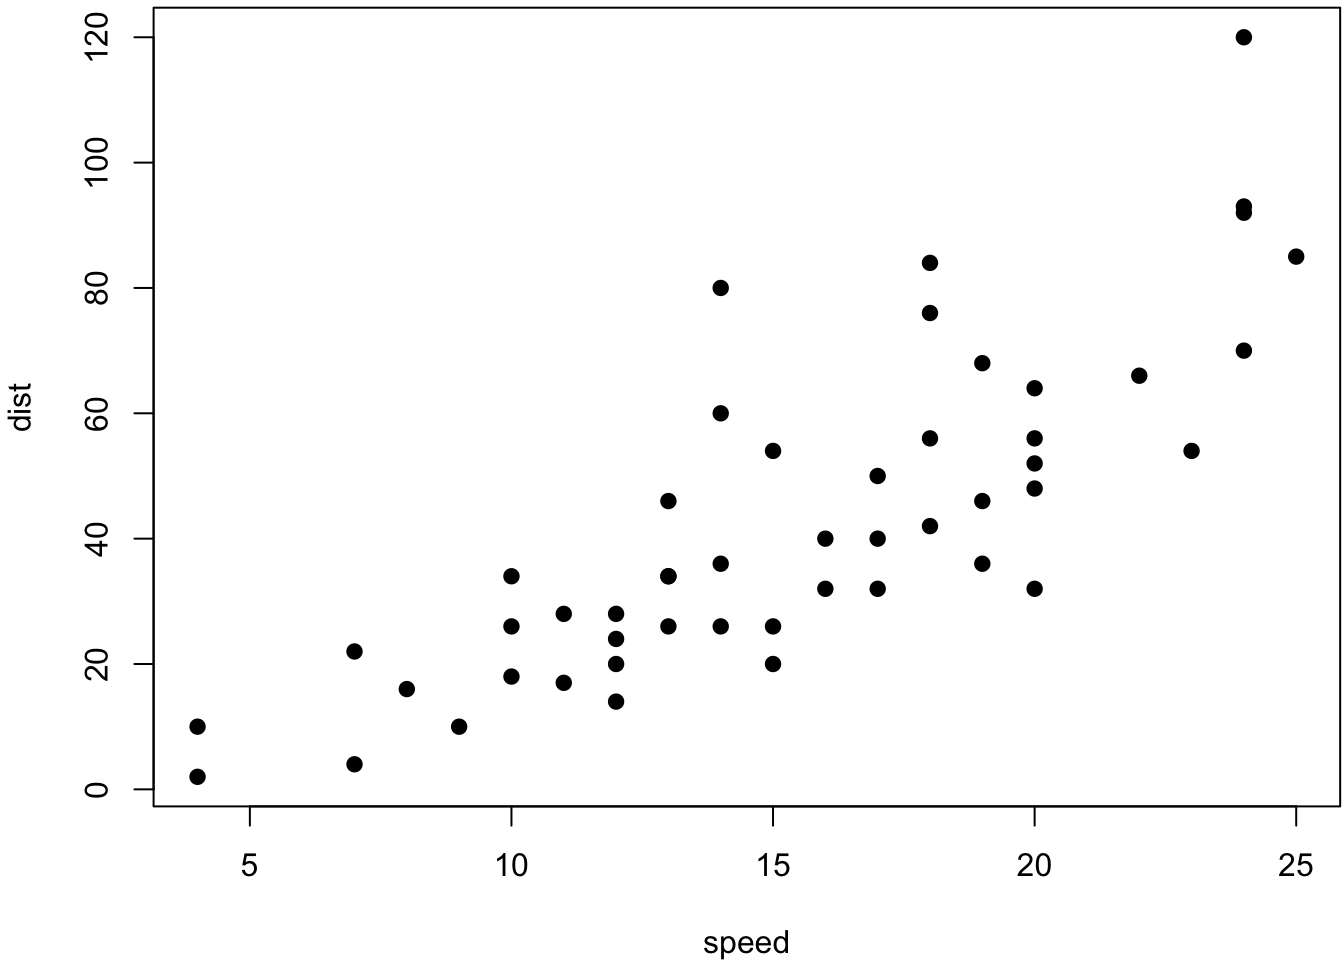
\includegraphics[width=1\linewidth]{bookdown-demo_files/figure-latex/c1-1}

Yet she does have a kind of respect for the creatures. ``Their behavior clearly works; there are a lot of harvester ant colonies out there, more every year,'' she observes. ``I deeply admire their harvester-ant-ness, the richness of their responses to a world so alien to me.''

\end{col}

\begin{col}{0.05\textwidth}
~

\end{col}

\begin{col}{0.45\textwidth}
Yet she does have a kind of respect for the creatures. ``Their behavior clearly works; there are a lot of harvester ant colonies out there, more every year,'' she observes. ``I deeply admire their harvester-ant-ness, the richness of their responses to a world so alien to me.''

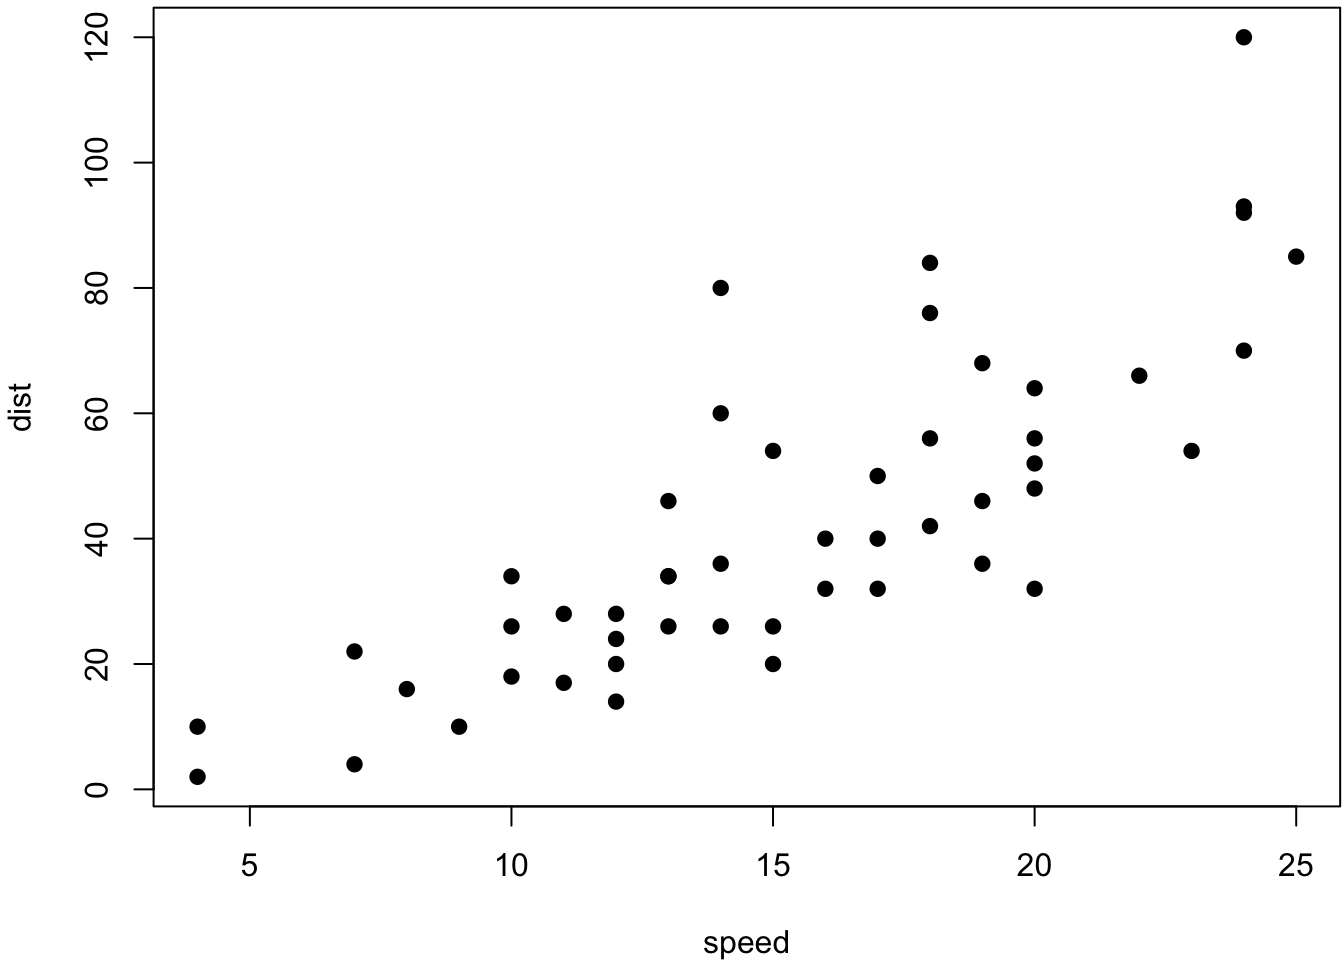
\includegraphics[width=1\linewidth]{bookdown-demo_files/figure-latex/c3-1}

\end{col}

\begin{longtable}[]{@{}l@{}}
\toprule
\endhead
\# random YAML comment \\
\bottomrule
\end{longtable}

  \bibliography{book.bib,packages.bib}

\end{document}
